\documentclass[aps,prapplied,reprint,superscriptaddress,longbibliography,nofootinbib]{revtex4-2}
\usepackage[utf8]{inputenc}
\usepackage[T1]{fontenc}
\usepackage{lmodern}
\usepackage{amsmath,amssymb,amsthm,bm}
\usepackage{graphicx}
\usepackage{booktabs}
\usepackage{siunitx}
\usepackage{algpseudocode}
\usepackage{xcolor}
\usepackage[colorlinks=true,linkcolor=blue!50!black,citecolor=blue!50!black,urlcolor=blue!50!black]{hyperref}
\usepackage{cleveref}

\newtheorem{proposition}{Proposition}
\newtheorem{lemma}{Lemma}
\newtheorem{theorem}{Theorem}
\theoremstyle{remark}
\newtheorem{remark}{Remark}

\newcommand{\T}{\mathsf{T}}
\newcommand{\R}{\mathbb{R}}
\newcommand{\E}{\mathbb{E}}
\newcommand{\tr}{\operatorname{tr}}
\newcommand{\vect}[1]{\bm{#1}}
\newcommand{\Sh}[1]{T_{#1}}
\newcommand{\yw}{\vect{y}_{\mathrm w}}
\DeclareMathOperator*{\argmax}{arg\,max}
\DeclareMathOperator*{\argmin}{arg\,min}

% generated by scripts/make_numbers.py -- do not edit
\newcommand{\resLinesLo}{1.7}
\newcommand{\resLinesHi}{2.8}
\newcommand{\resOFLo}{2.0}
\newcommand{\resOFHi}{12.4}
\newcommand{\resStatHi}{6.0}
\newcommand{\oracleGap}{0.03}
\newcommand{\gainLo}{1.2$\times$}
\newcommand{\gainMid}{3.3$\times$}
\newcommand{\gainHi}{4.5$\times$}
\newcommand{\gainMaxNoMorph}{15\%}
\newcommand{\resOFHiNoMorph}{3.2}
\newcommand{\resLinesHiNoMorph}{2.8}
\newcommand{\resStatHiNoMorph}{3.6}
\newcommand{\simAlpha}{99}
\newcommand{\simLoop}{27.5}
\newcommand{\simTau}{170}
\newcommand{\simIzero}{47.6}
\newcommand{\simPeakDrop}{2.0}
\newcommand{\sipcaIters}{3}
\newcommand{\smax}{12389}
\newcommand{\jitterTyp}{68}
\newcommand{\jitterRatioNoMorph}{7.0}
\newcommand{\jitterNoMorphLo}{18}
\newcommand{\jitterNoMorphHi}{30}
\newcommand{\jitterLowE}{30}
\newcommand{\crbLowE}{29}
\newcommand{\jitterPhaseHi}{3.6}
\newcommand{\crbHi}{3.3}
\newcommand{\jitterPhaseMaxRatio}{1.11}
\newcommand{\jitterMorphLo}{56}
\newcommand{\jitterMorphHi}{89}
\newcommand{\normBiasZero}{1.4}
\newcommand{\ofBiasZero}{0.36}
\newcommand{\mlBiasZero}{0.05}
\newcommand{\mlSpreadZero}{34\%}
\newcommand{\woodburyPrec}{$10^{-16}$}
\newcommand{\woodburySpeedup}{$2204$}
\newcommand{\rateLines}{688}
\newcommand{\rateOF}{2042}


\begin{document}

\title{Template-free optimal pulse processing for saturating microcalorimeters:
shift-invariant whitened PCA manifolds and Woodbury-accelerated non-stationary
maximum-likelihood estimation}
\author{To Chin Yu}
\affiliation{[Affiliation to be added]}
\date{\today}

\begin{abstract}
The optimal filter used for microcalorimeter pulses assumes a fixed template,
stationary noise and a known arrival time. Saturating transition-edge sensors
(TES) violate all three. We present a template-free estimator in three stages.
(A) Shift-invariant PCA in the noise-whitened domain learns a pulse subspace and
sub-sample arrival times by classification EM; it is exact because spectral
whitening commutes with Fourier shifts. (B) A spline manifold through the origin,
parameterised by whitened arc length (the cumulative matched-filter SNR, with unit
Fisher information), maps the coefficients to energy. (C) An energy-dependent,
low-rank covariance $R(E,t_0)=R_0+T_{t_0}G\Sigma(E)G^\T T_{t_0}^\T$ captures
pulse-correlated noise and shape fluctuations. The Woodbury identity and the
determinant lemma reduce the joint energy--time likelihood to about 12 dimensions.
We prove that shape fluctuations along the manifold tangent cannot be learned from
continuum data, but can be learned from mono-energetic clusters without knowing
their energies. On a physical simulation of a saturating TES, tested on held-out
lines, the estimator reaches \resLinesLo--\resLinesHi\,eV FWHM from 1 to 11\,keV,
against \resOFLo--\resOFHi\,eV for a plain optimal filter. Most of that gap is also
closed by tuned empirical corrections. Against the best of four prior-art
pipelines, the estimator is level at low energy and up to \impBestTopMorph\% better
at 11\,keV, within \oracleGap\,eV of an oracle. On real NIST TES data dominated by
one line, it improves on phase-corrected filtering with projector decorrelation by
\realImpBest\%. A label-free sampling-phase correction brings arrival times close to the
Cramér--Rao bound, but it needs about $10^5$ records per energy. An
open-source Python implementation accompanies the paper.
\end{abstract}

\maketitle

%==========================================================================
\section{Introduction}
\label{sec:intro}

Thermal microcalorimeters such as transition-edge sensors (TES), metallic magnetic
calorimeters and thermal kinetic-inductance detectors reach energy resolutions of a
few eV at keV energies~\cite{Moseley1984,IrwinHilton2005}. The standard estimator is
the optimal filter (OF)~\cite{Szymkowiak1993,Fowler2016practice}: a frequency-domain
matched filter that is the minimum-variance unbiased amplitude estimator if (i) every
pulse is a scaled copy of one template, (ii) the noise is additive, Gaussian and
stationary, and (iii) the arrival time is known. Real detectors break each
assumption. As a TES is driven up its transition, the pulse shape evolves with
energy and eventually saturates. The Johnson and thermal-fluctuation noise depend on
the instantaneous resistance and temperature, so the noise during a pulse differs
from the baseline noise. Arrival times are continuous, which leads to sampling-phase
(``arrival-time'') effects~\cite{Fowler2016practice}. Position-dependent
thermalisation adds shape variation that is not a function of energy.

Three lines of work address these effects. \emph{Calibration-based non-linear and
non-stationary filters} estimate energy-dependent templates and full covariance
matrices at calibration energies and interpolate between
them~\cite{Fixsen2002,Fixsen2004,Shank2014,Fixsen2014,Peille2016}. Fixsen
\emph{et al.}~\cite{Fixsen2014} gave this a differential-geometric interpretation, and
Fowler \emph{et al.}~\cite{Fowler2017tangent} showed that filtering along the
\emph{tangent} of the energy curve of mean pulses improves on the OF. These methods
are the most accurate known. Their full-rank covariances, however, cost
$\mathcal O(N^3)$ per energy and need many calibration pulses, a burden that led
the Athena X-IFU study to judge them impractical~\cite{Peille2016}. \emph{Empirical
corrections} applied to the OF output are the practitioner's standard. They include
arrival-phase and drift corrections~\cite{Fowler2016practice} and decorrelation
against residual ``projector'' components, as implemented in NIST's MASS
software~\cite{mass}. In dark-matter detectors, pulse-shape variation is treated as
non-stationary noise added to the OF covariance~\cite{CDMSlite2018,Albakry2026}.
\emph{Data-driven subspace methods} use principal component analysis (PCA) or
singular value decomposition (SVD) of the
records~\cite{deVries2016,Yan2016,Busch2016,Alpert2016,Fowler2018nonlinear,Fowler2020rpca,Miller2021,Yu2019}
and, more recently, neural networks~\cite{Ichinohe2022,Albakry2026}. In earlier
work~\cite{Yu2019} we proposed a template-free estimator based on a weighted
EM-PCA~\cite{Roweis1998,Bailey2012} of a phase-differenced Fourier transform that is
invariant to arrival time. That construction discards arrival-time information by
design, and its pulse-height estimator, the norm of the coefficient vector, is
rectified at low signal-to-noise ratio.

This paper combines the three lines into one likelihood. It learns the pulse family
from unlabelled data, as the subspace methods do. It models energy-dependent,
non-stationary noise and shape fluctuations, as the calibration-based filters do,
but with a low-rank parameterisation that is cheap to evaluate and needs few
calibration pulses. It replaces the empirical corrections with a joint
energy--time likelihood. \Cref{sec:related} positions each component against
prior work. The contributions are:
\begin{enumerate}
\item \textbf{Shift-invariant whitened PCA} (\cref{sec:stageA}). We show that the
symmetric spectral whitening operator $R_0^{-1/2}$ commutes with fractional Fourier
shifts, whereas a Cholesky factor of the Toeplitz covariance does not
(\cref{lem:commute}). In the whitened domain, alignment (E-step) and subspace
learning (M-step) of a transformation-invariant EM~\cite{FreyJojic2003} become
exact operations at sub-sample resolution. We prove monotone convergence
(\cref{prop:monotone}) and show that the noise does not bias the learned subspace
(\cref{prop:unbiased}). We also prove that a subspace containing the time
derivative of the pulse carries no timing information (\cref{prop:derivative}).
\item \textbf{Arc-length spline manifold} (\cref{sec:stageB}). A data-driven
realisation of the energy curve of
Refs.~\cite{Fixsen2014,Fowler2017tangent,Fowler2018nonlinear}: a P-spline graph
through the origin in whitened coefficient space, parameterised by whitened arc
length. In that parameter the Fisher information is one, and the estimate is
unbiased at zero energy (\cref{prop:rician}).
\item \textbf{Low-rank, Woodbury-accelerated non-stationary ML} (\cref{sec:stageC}).
We use an energy-dependent covariance on the signal subspace plus a few
learned residual modes. With it, the exact non-stationary log-likelihood reduces to
$K_b\ll N$ dimensions (\cref{thm:woodbury}), as for low-rank Gaussian processes in
pulsar timing~\cite{vanHaasteren2014,Lentati2017}. We prove an identifiability
result (\cref{prop:identifiability}): fluctuations along the manifold tangent
cannot be learned from unlabelled continuum events, but can be learned from
mono-energetic clusters, without knowing their energies.
\item \textbf{A physical simulation study} (\cref{sec:sim,sec:results}) of a
saturating TES, with held-out test lines. We compare against the OF, against OF
with phase correction and residual-projector decorrelation (the practitioner's
standard), against a stationary secant (tangent) filter, against an
energy-dependent full-covariance filter, and against an oracle Gaussian model.
\item \textbf{Open-source software}: a tested Python package with a
scikit-learn-like interface (\cref{app:software}).
\end{enumerate}

%==========================================================================
\section{Related work}
\label{sec:related}

\paragraph{Shift-invariant subspace learning.} Jointly inferring per-sample shifts
and learning components by EM is established in machine learning, as
transformation-invariant clustering and factor analysis with FFT-computed
shifts~\cite{FreyJojic2003,Kannan2002}. In neuroimaging it appears as shift-invariant
decompositions with frequency-domain delays~\cite{Morup2008}. In functional data
analysis it is registration combined with PCA~\cite{KneipRamsay2008}, and in
cryo-electron microscopy it is multi-reference alignment~\cite{Sigworth1998}. Among
microcalorimeter methods, Ref.~\cite{Yu2019} linearised the shift in a
phase-differenced Fourier domain instead of estimating it. NIST's MASS
builds SVD ``projector'' bases in which the arrival time enters as a derivative
component~\cite{mass,Fowler2016practice,Fowler2020rpca}. Alpert
\emph{et al.}~\cite{Alpert2016} built an SVD single-pulse model with sub-sample
arrival times for pile-up rejection. We found no microcalorimeter method that
alternates sub-sample alignment with re-learning a noise-whitened basis. Our
additions to the generic algorithm are the whitening that makes it exact
(\cref{lem:commute}), continuous shifts and the timing degeneracy of
\cref{prop:derivative}.

\paragraph{Energy curves and manifolds.} The pulse family of a non-linear detector
is a curve in record space~\cite{Fixsen2014}. Tangent filtering uses its local
tangent from energy-specific mean pulses~\cite{Fowler2017tangent}. Fowler
\emph{et al.}~\cite{Fowler2018nonlinear} fitted cubic splines to linear-subspace
components as functions of an energy estimator. Yan \emph{et al.}~\cite{Yan2016} and
Miller \emph{et al.}~\cite{Miller2021} mapped PCA coefficients to energy with the
help of calibration lines. Our curve is learned without labels as a graph through
the origin in \emph{whitened} coefficient space. Its whitened arc length equals the
cumulative matched-filter SNR, which gives the parameter a statistical meaning
(unit Fisher information) and makes the low-energy estimate unbiased.

\paragraph{Non-stationary noise.} Energy-dependent full covariances in a least-squares
fit go back to Fixsen \emph{et al.}~\cite{Fixsen2002,Fixsen2004}, with simulated
covariances in Ref.~\cite{Shank2014} and calibration-line covariances interpolated in
energy in Athena's SIRENA software~\cite{Peille2016}. SuperCDMS add the covariance of
template residuals, aligned to the arrival time, to the noise~\cite{CDMSlite2018},
and treat the shape uncertainty of PCA templates as non-stationary
noise~\cite{Albakry2026}. These covariances are full-rank, or their modes are fitted
as free amplitudes. A white-plus-low-rank covariance evaluated with the Woodbury
identity and the determinant lemma is standard for Gaussian-process noise in
pulsar timing~\cite{vanHaasteren2014}. Lentati \emph{et al.}~\cite{Lentati2017} fit
arrival times jointly with stochastic profile variations, and Moore and
Gair~\cite{MooreGair2014} marginalise waveform-model error as a covariance in
gravitational-wave inference. To our knowledge, a learned, low-rank, continuous
$\Sigma(E)$ inside a joint energy--time likelihood has not been used for
cryogenic detectors. Nor have we found the identifiability statement of
\cref{prop:identifiability}, although its geometry is that of
Refs.~\cite{Fixsen2014,Fowler2017tangent}.

\paragraph{Software.} The most complete open practitioner pipelines are NIST's
MASS (whitened OF, projectors, phase and drift corrections)~\cite{mass} and
SuperCDMS's QETpy (OF variants, including non-linear and multi-template
filters)~\cite{qetpy}. SIRENA implements the covariance-matrix methods of
Ref.~\cite{Peille2016}. None implements the alternating shift-invariant learning, the
whitened arc-length manifold or the low-rank joint likelihood. A detailed survey is
included with the code (\texttt{paper/PRIOR\_ART.md}).

%==========================================================================
\section{Signal model and notation}
\label{sec:model}

A record $\vect y\in\R^N$ sampled at rate $f_s$ is modelled as
\begin{equation}
\vect y = \Sh{t_0}\,\vect m(E,\eta) + \vect n ,
\label{eq:model}
\end{equation}
where $\vect m(E,\eta)$ is the noise-free pulse for deposited energy $E$ and
nuisance morphology $\eta$ (e.g.\ absorption position), $t_0$ is the arrival time
in samples, and $\vect n$ is zero-mean Gaussian noise. Let $F$ be the unitary DFT.
The (band-limited, circular) shift operator is
\begin{equation}
\Sh{\tau} = F^{H}\operatorname{diag}\!\left(e^{-2\pi i k\tau/N}\right)F, \qquad
(\Sh{\tau}\vect x)(t)=x(t-\tau),
\end{equation}
with the Nyquist bin removed so that $\Sh\tau$ maps real signals to real signals and
is orthogonal on the remaining band for any real $\tau$. Its generator is the
spectral derivative $D=F^H\operatorname{diag}(2\pi i k/N)F$, with
$\Sh{\tau}=e^{-\tau D}$ and $D^\T=-D$. Baseline noise is approximated by a
circulant covariance $R_0=F^H\Lambda F$, with $\Lambda=\operatorname{diag}(\lambda_k)$
estimated from pulse-free records as $\lambda_k=\E|Y_k|^2/N$. This approximation
is asymptotically equivalent to the Toeplitz covariance~\cite{Gray2006} and is
standard in OF practice~\cite{Szymkowiak1993}. We exclude the DC bin (baseline
offset) and the Nyquist bin, which leaves $N-2$ real degrees of freedom.

\begin{lemma}[Whitening commutes with shifts]\label{lem:commute}
Let $W=R_0^{-1/2}=F^H\Lambda^{-1/2}F$. Then $W\Sh\tau=\Sh\tau W$ for all
$\tau\in\R$, and $W\vect n$ is white with unit variance on the analysis band. If $G$
is any other whitening matrix ($GR_0G^\T=I$), then $G=QW$ with $Q$ orthogonal, and
$G$ commutes with all $\Sh\tau$ if and only if $Q$ is diagonalised by $F$. In
particular, the inverse Cholesky factor $L_0^{-1}$ of a non-circulant Toeplitz
$R_0$ does not commute with shifts.
\end{lemma}
\begin{proof}
$W$ and $\Sh\tau$ are both diagonal in the Fourier basis. For the second statement,
$(GW^{-1})(GW^{-1})^\T=GR_0G^\T=I$, so $Q=GW^{-1}$ is orthogonal, and $Q$ commutes
with the full family $\{\Sh\tau\}$ iff it is a function of $D$, i.e.\ diagonal in
$F$. A lower-triangular $L_0^{-1}$ is not circulant unless $R_0$ is diagonal.
\end{proof}

All subsequent processing works with whitened records $\yw=W\vect y$. A delay of the
raw record is the same delay of the whitened record, so a shifted pulse remains a
shifted pulse after whitening. This is the property that makes the methods below
exact rather than approximate.

%==========================================================================
\section{Stage A: shift-invariant whitened PCA}
\label{sec:stageA}

\subsection{Model and objective}
In the whitened domain we model the pulses of a training set as lying in an unknown
$K$-dimensional subspace with orthonormal basis $B\in\R^{K\times N}$ ($BB^\T=I$):
\begin{equation}
\yw^{(j)} = \Sh{\tau_j} B^\T \vect a_j + \vect\varepsilon_j,
\qquad \vect\varepsilon_j\sim\mathcal N(0,I).
\end{equation}
The amplitudes $\vect a_j$ profile out as $\hat{\vect a}_j=B\Sh{-\tau_j}\yw^{(j)}$.
The negative log-likelihood is then $\sum_j\|\yw^{(j)}\|^2-J(B,\{\tau_j\})$ with
captured power
\begin{equation}
J(B,\{\tau_j\})=\sum_j \left\|B\,\Sh{-\tau_j}\yw^{(j)}\right\|^2 .
\label{eq:J}
\end{equation}
We maximise $J$ by alternating over the latent shifts and the basis. This is a hard
(classification) EM, a shift-invariant analogue of EM-PCA~\cite{Roweis1998,TippingBishop1999}.

\subsection{E-step: phase-coherent cross-correlation}
For fixed $B$, each $\tau_j$ maximises $g_j(\tau)=\|\vect x_j(\tau)\|^2$, where
$x_{jk}(\tau)=\langle\vect b_k,\Sh{-\tau}\yw^{(j)}\rangle$. Writing $\hat{\cdot}$
for the real FFT and $w_k\in\{1,2\}$ for the multiplicity of each half-spectrum
bin,
\begin{equation}
x_{jk}(\tau)=\frac1N\sum_{k'} w_{k'}\,\Re\!\left[\overline{\hat b_{k,k'}}\,
\hat y_{j,k'}\,e^{2\pi i k'\tau/N}\right].
\label{eq:xcorr}
\end{equation}
For all integer lags this is a cross-correlation, computed with one inverse FFT per
basis vector. The maximum is then refined to sub-sample precision with guarded
Newton steps on the exact band-limited function~\eqref{eq:xcorr}. Its
$\tau$-derivatives follow analytically by multiplying the summand by
$(2\pi i k'/N)^m$, at $\mathcal O(KN)$ cost per step. Unlike up-sampling or
parabolic interpolation, this optimises the true likelihood, so the estimate
inherits the asymptotic efficiency of maximum likelihood.

\subsection{M-step: counter-rotation and SVD}
For fixed $\{\tau_j\}$, $J$ is maximised by the top-$K$ right singular vectors of the
matrix $X$ whose rows are the counter-rotated records $\Sh{-\tau_j}\yw^{(j)}$. The
counter-rotation is a phase ramp in the frequency domain. We compute the $N\times N$
scatter matrix $X^\T X$ and its eigendecomposition.

\begin{proposition}[Whitened noise does not bias the subspace]\label{prop:unbiased}
If $\yw^{(j)}=\Sh{\tau_j}\vect\mu_j+\vect\varepsilon_j$ with $\vect\varepsilon_j$
white and the shifts are known, then
$\E[X^\T X]/n=\frac1n\sum_j\vect\mu_j\vect\mu_j^\T+P$, where $P$ projects onto the
analysis band. The noise term is isotropic, so the eigenvectors are those of the
noise-free scatter matrix.
\end{proposition}
\begin{proof}
$\Sh{-\tau_j}$ is orthogonal and commutes with $P$, so
$\E[\Sh{-\tau_j}\vect\varepsilon_j\vect\varepsilon_j^\T\Sh{-\tau_j}^\T]=P$.
\end{proof}
The proposition fails without whitening: coloured noise adds a non-isotropic term
$R_0$ and tilts the subspace toward the noise-dominated frequencies. With
\emph{estimated} shifts, low-SNR records are aligned partly to their own noise. This
is the ``template from noise'' bias known from cryo-electron
microscopy~\cite{Sigworth1998,Henderson2013}. We therefore learn $B$ only from
records whose whitened excess power exceeds $\mathrm{SNR}_{\min}^2$. All records
are still aligned and projected.

\subsection{Convergence, gauge and a timing degeneracy}

\begin{proposition}[Monotonicity]\label{prop:monotone}
Let the E-step maximise
$J_r=\sum_j\|B_{1:r}\Sh{-\tau_j}\yw^{(j)}\|^2$ over $\tau_j$ for the leading
$r\le K$ basis vectors, and let the M-step take the top-$K$ singular vectors. Then
$J_r$ is non-decreasing over the iterations.
\end{proposition}
\begin{proof}
The E-step maximises $J_r$ for fixed $B$. The top-$r$ right singular vectors
maximise $\sum_j\|B_{1:r}\vect x_j\|^2$ over all $r$-frames (Ky Fan), and they are
the first $r$ of the top-$K$ singular vectors.
\end{proof}

The model is invariant under a common shift
$(B,\tau_j)\mapsto(\Sh{\delta}B,\tau_j+\delta)$. We fix this gauge by setting the
median arrival time of the training set to zero after every iteration; this leaves
$J_r$ unchanged. The choice of $r$ is governed by the following result.

\begin{proposition}[A subspace containing the pulse derivative carries no timing
information]\label{prop:derivative}
Let $P_B$ be the projector onto $\operatorname{span}(B)$ and $g(\tau)=\|P_B
\Sh{-\tau}\vect y\|^2$. At a point where $\vect z=\Sh{-\tau}\vect y\in
\operatorname{span}(B)$,
\begin{equation}
g''(\tau) = -2\,\|(I-P_B)\,D\vect z\|^2 .
\end{equation}
The curvature of the profile likelihood in $\tau$, and so the Fisher information
of the subspace estimator of $t_0$, comes only from the part of the time
derivative of the pulse that lies \emph{outside} the subspace.
\end{proposition}
\begin{proof}
$\frac{d}{d\tau}\vect z=D\vect z$. Then
$g'=2\vect z^\T P_BD\vect z$ and
$g''=2(D\vect z)^\T P_B(D\vect z)+2\vect z^\T P_BD^2\vect z$. With $P_B\vect z=\vect z$
and $D^\T=-D$, the second term equals $-2\|D\vect z\|^2$, and
$\|D\vect z\|^2-\|P_BD\vect z\|^2=\|(I-P_B)D\vect z\|^2$.
\end{proof}
A free $K$-dimensional subspace learned from jittered data tends to absorb the
derivative direction, since it explains small shifts linearly, and its E-step then
becomes ill-posed. We observed exactly this for $K\ge3$ with $r=K$ (timing
scatter of a full sample). With $r=1$ the alignment uses only the leading,
mean-pulse direction $\vect b_1$. Since $\langle\vect b_1,D\vect b_1\rangle=0$,
\cref{prop:derivative} then gives the classical OF timing information
$a_1^2\|D\vect b_1\|^2$. The remaining $K-1$ directions describe shape variation
\emph{after} alignment. The final timing estimate comes from the manifold-constrained
likelihood of Stage C, where the pulse family is one-dimensional and cannot absorb
shifts.

%==========================================================================
\section{Stage B: arc-length spline manifold}
\label{sec:stageB}

\subsection{Representation}
The aligned coefficients $\vect a_j=B\Sh{-\tau_j}\yw^{(j)}\in\R^K$ have unit
isotropic noise (\cref{prop:unbiased}) and concentrate near a curve, the image of
the energy axis. Let $\vect e$ be the leading uncentred principal direction of
$\{\vect a_j\}$ (the mean-pulse direction), $u=\langle\vect e,\vect a\rangle$, and
let the columns of $\tilde W$ span the orthogonal complement. We represent the
curve as the graph
\begin{equation}
\vect c(u)=\vect e\,u+\tilde W\,u\,\vect h(u),\qquad \vect h=\text{cubic P-spline},
\end{equation}
fitted by penalised least squares~\cite{EilersMarx1996}. The penalty is selected by
generalised cross-validation~\cite{CravenWahba1979}. Three properties are built in.
The curve passes through the origin (a zero-energy event is no pulse) and is linear
for small signals. It is continued linearly for $u<0$ and tangentially beyond the
data. Being a graph over $u$, it cannot fold back on itself. Free-form principal
curves~\cite{HastieStuetzle1989}, which we tried first, did fold back in sparse,
strongly saturated regions.

\paragraph{Mono-energetic clusters and the secant fallback.} The scatter of records
within a mono-energetic line is, by definition, not along the energy direction
(\cref{prop:identifiability}). Left in the fit, it can tilt the curve's tangent
toward the dominant within-line fluctuation, which is typically a sampling-phase
mode. After a first pass, we therefore refit the curve with each cluster found in
the spectrum (\cref{sec:identifiability}) replaced by its mean, weighted by its
size. If too few records lie outside the clusters to determine the curvature (we
require 30 per spline coefficient), the curve is taken as the shape-preserving
secant through the origin and the cluster means. This is the learned analogue of
the secant or tangent filter~\cite{Fowler2017tangent}, and the case of real data
dominated by a single line (\cref{sec:realdata}).

\subsection{Arc length and the Fisher information}
We re-parameterise by whitened arc length,
$s(u)=\int_0^u\|\vect c'(v)\|\,dv$, so that $\|d\vect c/ds\|=1$. Under stationary
noise with known alignment, $\vect a=\vect c(s)+\vect\varepsilon$ with
$\vect\varepsilon\sim\mathcal N(0,I_K)$, the Fisher information is
$I_{ss}=\|d\vect c/ds\|^2=1$, so
\begin{equation}
\sigma_s\ge1,\qquad \sigma_E \ge \left|\frac{dE}{ds}\right|,\qquad
\mathrm{FWHM}_E\ge 2.355\left|\frac{dE}{ds}\right| .
\end{equation}
In the linear regime, $\vect c(s)=s\vect e$ and $s=\langle\vect e,\vect a\rangle$ is
the OF amplitude divided by its baseline resolution, i.e.\ the matched-filter SNR.
The arc length is therefore the natural generalisation of the OF SNR to evolving
pulse shapes. The ML estimate given the alignment is the closest point of the curve.

When the arrival time is estimated jointly, $\partial_s\vect\mu=B^\T\vect c'$ and
$\partial_\tau\vect\mu=-D\vect\mu$ with $\vect\mu=B^\T\vect c(s)$. In the linear
regime $\langle\vect c',D\vect\mu\rangle\propto\langle\vect b_1,D\vect b_1\rangle=0$
and energy and time are Fisher-orthogonal. When the shape evolves with energy they
are not: the cross term is the information-geometric origin of time walk, and the
CRB on $s$ inflates by $1/(1-\rho^2)$, where $\rho$ is the Fisher correlation
coefficient. The joint fit of Stage C accounts for this automatically.

\subsection{No rectification at low energy}
\begin{proposition}[Rectification of the coefficient norm]\label{prop:rician}
If $\vect a\sim\mathcal N(\vect c,I_K)$ then $\E\|\vect a\|^2=\|\vect c\|^2+K$ and,
for $\vect c=0$, $\|\vect a\|$ follows a $\chi_K$ distribution with mean
$\sqrt2\,\Gamma(\frac{K+1}2)/\Gamma(\frac K2)>0$. The manifold coordinate with
linear continuation through the origin satisfies $\hat s=\langle\vect e,\vect
a\rangle\sim\mathcal N(0,1)$ for $\vect c=0$, to the extent that the curve is
straight within a few noise units of the origin, and is unbiased.
\end{proposition}
The norm estimator of Ref.~\cite{Yu2019} therefore has an energy-dependent bias of
order $K/(2\|\vect c\|)$ that vanishes only at high SNR, plus a non-linear response
near threshold. The manifold coordinate has neither.

\subsection{Energy scale}
The manifold, and hence $s$, is learned without labels. The map $E(s)$ is monotone
and, in the linear regime, proportional, but its curvature at high energy cannot be
recovered from pulse shapes alone. We fit it with a shape-preserving cubic
interpolant through the origin and the positions of known lines, as for any
non-linear detector. This is the sense in which the method is template-free but
not calibration-free.

%==========================================================================
\section{Stage C: Woodbury-accelerated non-stationary maximum likelihood}
\label{sec:stageC}

\subsection{Covariance model}
Pulse-correlated noise has several sources: resistance- and temperature-dependent
Johnson and phonon noise, residual shape fluctuations such as position dependence,
and the shape distortion caused by sampling a pulse that is not band-limited at a
random sub-sample phase. We model all of them by a low-rank, energy-dependent excess
covariance. In the whitened frame aligned to the pulse,
\begin{equation}
\yw \sim \mathcal N\!\left(\Sh{\tau}\vect\mu(s),\; I+\Sh{\tau}V^\T\Sigma(s)V\Sh{\tau}^\T\right),
\label{eq:ns-model}
\end{equation}
with $V\in\R^{K_v\times N}$ orthonormal and $\Sigma(s)$ a symmetric $K_v\times K_v$
matrix with $\Sigma(0)=0$ and eigenvalues $>-1$. We take
$V=\left[\begin{smallmatrix}B\\V_r\end{smallmatrix}\right]$: the signal basis plus
$K_n$ residual modes $V_r$ orthogonal to it, so that $K_v=K+K_n$. Including $B$
matters. The energy tangent $B^\T\vect c'(s)$ lies in $\operatorname{span}(B)$, and
the in-pulse noise along these directions can differ from baseline in either sign.
A model built only from the largest residual modes misses this
(\cref{sec:results}). In the raw domain,
using \cref{lem:commute}, this is
\begin{equation}
R(E,t_0)=R_0+\Sh{t_0}\,G\,\Sigma(E)\,G^\T\,\Sh{t_0}^\T,\qquad G=R_0^{1/2}V^\T ,
\end{equation}
which is the form of the original proposal. Because $\Sh{t_0}$ commutes with $R_0$,
the Gram matrix $G^\T\Sh{t_0}^\T R_0^{-1}\Sh{t_0}G=VV^\T=I$ does not depend on
$t_0$. This is why the shift does not spoil the low-rank algebra. Negative
eigenvalues of $\Sigma$ are allowed: in a saturating TES the noise during a pulse
can be \emph{lower} than the baseline noise (\cref{sec:results}).

\subsection{Reduction to $K_b$ dimensions}
\begin{theorem}\label{thm:woodbury}
Let $\tilde B\in\R^{K_b\times N}$ be an orthonormal basis of
$\operatorname{span}(B,V)$, $\vect x(\tau)=\tilde B\Sh{-\tau}\yw$,
$\vect m(s)=\tilde BB^\T\vect c(s)$, $Q=\tilde BV^\T$ and
$M(s)=\Sigma(s)\,[I+\Sigma(s)]^{-1}$. Then
\begin{multline}
-2\log L(s,\tau) = \|\yw\|^2-\|\vect x\|^2+\|\vect x-\vect m\|^2\\
-(\vect x-\vect m)^\T QMQ^\T(\vect x-\vect m)+\log\det\!\left(I+\Sigma\right)
+\text{const}.
\label{eq:woodbury}
\end{multline}
\end{theorem}
\begin{proof}
Let $U=\Sh{\tau}V^\T$, which has orthonormal columns. The Woodbury
identity~\cite{Woodbury1950,Hager1989} gives
$(I+U\Sigma U^\T)^{-1}=I-U(\Sigma^{-1}+I)^{-1}U^\T=I-UMU^\T$; the last form holds
also for singular $\Sigma$. The determinant lemma gives
$\det(I+U\Sigma U^\T)=\det(I+\Sigma U^\T U)=\det(I+\Sigma)$. For the residual
$\vect r=\yw-\Sh\tau\vect\mu$, orthogonality of $\Sh{\tau}$ gives
$\vect r^\T\vect r=\|\Sh{-\tau}\yw-\vect\mu\|^2$ and
$U^\T\vect r=V(\Sh{-\tau}\yw-\vect\mu)$. Decompose $\Sh{-\tau}\yw$ into its
projection $\tilde B^\T\vect x$ and an orthogonal remainder. Since
$\vect\mu=\tilde B^\T\vect m$ and $V=Q^\T\tilde B$, we get
$\|\Sh{-\tau}\yw-\vect\mu\|^2=\|\yw\|^2-\|\vect x\|^2+\|\vect x-\vect m\|^2$ and
$V(\Sh{-\tau}\yw-\vect\mu)=Q^\T(\vect x-\vect m)$.
\end{proof}

\paragraph{Cost.} Whitening and one real FFT cost $\mathcal O(N\log N)$ per record.
The aligned projections $\vect x(\tau)$ cost $\mathcal O(K_b N\log N)$ for all
integer lags at once, or $\mathcal O(K_bN)$ at one continuous $\tau$ with its first
two derivatives (\cref{eq:xcorr}). The rest of~\eqref{eq:woodbury} costs
$\mathcal O(K_bK_v+K_v^3)$ per $(s,\tau)$. A dense non-stationary filter instead
needs an $\mathcal O(N^3)$ factorisation of $R(E,t_0)$ for every energy, and for
every $t_0$ if the shift is applied to the covariance. Alternatively it can
precompute inverses on a grid at $\mathcal O(N^2)$ memory per node. Here $K_b=K_v=K+K_n\approx 12$,
against $N=1024$.

\subsection{Learning $V$ and $\Sigma(s)$ and what is identifiable}
\label{sec:identifiability}
Given Stage A/B estimates $(\hat s_j,\hat\tau_j)$, the aligned whitened records
$\vect z_j=\Sh{-\hat\tau_j}\yw^{(j)}$ supply residuals. We take $V_r$ as the top-$K_n$
eigenvectors of the pooled residual covariance projected onto the complement of
$\operatorname{span}(B)$. $\Sigma$ is estimated at knots $s_b$ as
$V\widehat{\operatorname{Cov}}_b(\vect z)V^\T-I$, a $K_v\times K_v$ matrix that is
well determined from a few hundred events, with $\Sigma(0)=0$, and
interpolated with a monotone cubic (PCHIP) per entry, with eigenvalues clipped at
$-\frac12$. The definition of the residual matters.

\begin{proposition}[Tangential fluctuations are not identifiable from continuum
data]\label{prop:identifiability}
Let records at energy $E$ fluctuate as $\vect\mu(s)+\xi\,\vect d$ with $\xi$
zero-mean and $\vect d=\alpha\,\vect\mu'(s)+\vect d_\perp$,
$\vect d_\perp\perp\vect\mu'(s)$. To first order in $\xi$, the distribution of
records is the same as that of a model with fluctuation $\xi\vect d_\perp$ and an
energy distribution $p(s)$ convolved with the law of $\alpha\xi$. If $p$ is unknown
and smooth (a continuum), the two models cannot be distinguished. If $p$ has atoms
(mono-energetic lines), the convolution is detectable and $\alpha$ is identified.
\end{proposition}
\begin{proof}
$\vect\mu(s)+\xi\alpha\vect\mu'(s)+\xi\vect d_\perp=\vect\mu(s+\alpha\xi)+\xi\vect
d_\perp+\mathcal O(\xi^2)$.
\end{proof}
Consequently, residuals about the fitted curve, $\vect z_j-B^\T\vect c(\hat s_j)$,
reveal only $\vect d_\perp$; we call this label-free variant ``curve''. Since
$\vect d_\perp\perp\vect\mu'$, down-weighting it does not change the energy
estimate to first order. The ``line-aware'' variant instead takes residuals about
the mean of each mono-energetic cluster, found as a peak of the histogram of
$\hat s$. This reveals the full $\vect d$, including the tangential part that
broadens the line. The resulting ML estimate is the oblique projection along
$\vect d$ (cf.\ Ref.~\cite{Fixsen2014}). It is a learned, multi-dimensional
generalisation of the empirical rise-time and arrival-phase corrections used in
practice~\cite{Fowler2016practice}. No energies are needed for this step, only the
existence of sharp lines. Lines with a poor peak-to-continuum ratio contaminate the
cluster covariance with genuine energy spread.

\subsection{Optimisation and Cramér--Rao bounds}
We maximise~\eqref{eq:woodbury} jointly over $(s,\tau)$ with a Levenberg-damped
$2\times2$ Newton iteration and backtracking, vectorised over records. Derivatives
in $\tau$ are analytic, via~\eqref{eq:xcorr}; derivatives in $s$ are central
differences of the $K_b$-dimensional expression. The iteration starts from the
Stage A/B estimates. The Fisher information of the learned model
is~\cite{Kay1993}
\begin{gather}
I_{ij}=\partial_i\vect\mu^\T R_w^{-1}\partial_j\vect\mu+\tfrac12\tr\!\left(R_w^{-1}
\partial_iR_w\,R_w^{-1}\partial_jR_w\right),\\
\partial_\tau R_w=-(DV^\T\Sigma V+V^\T\Sigma VD^\T),
\end{gather}
with $\partial_s R_w=V^\T\Sigma'(s)V$. We report bounds with and without the
covariance term, because the latter relies on the exact energy dependence of
$\Sigma$.

\Cref{alg:pipeline} summarises the procedure.

\begin{figure}[t]
\small
\begin{algorithmic}[1]
\Require pulse records $\{\vect y_j\}$, pulse-free records, $K$, $K_n$, number of lines
\State $\lambda_k\gets$ periodogram of pulse-free records; $\yw\gets W\vect y$ \Comment{\cref{lem:commute}}
\State $B\gets$ top-$K$ SVD of $\{\yw^{(j)}\}$ with $\mathrm{SNR}>\mathrm{SNR}_{\min}$
\Repeat \Comment{Stage A}
  \State $\tau_j\gets\argmax_\tau\|B_{1:r}\Sh{-\tau}\yw^{(j)}\|^2$ (FFT lags, then Newton)
  \State $B\gets$ top-$K$ right singular vectors of $\{\Sh{-\tau_j}\yw^{(j)}\}$; re-gauge
\Until{$J_r$ converged}
\State $\vect a_j\gets B\Sh{-\tau_j}\yw^{(j)}$; fit spline graph $\vect c$; $s\gets$ arc length \Comment{Stage B}
\State $(s_j,\tau_j)\gets$ stationary ML (\cref{eq:woodbury} with $\Sigma=0$)
\State clusters $\gets$ peaks of $\{s_j\}$; $V,\Sigma(s)\gets$ cluster residual covariances \Comment{Stage C}
\State $(s_j,\tau_j)\gets\argmin$ \cref{eq:woodbury}; $E_j\gets E(s_j)$ from reference lines
\end{algorithmic}
\caption{The template-free pulse processing algorithm.}\label{alg:pipeline}
\end{figure}

%==========================================================================
\section{Physical simulation}
\label{sec:sim}

To test the method on effects that are physical rather than put in by hand, we
integrate the coupled electro-thermal Langevin equations of a voltage-biased
one-body TES~\cite{IrwinHilton2005}:
\begin{align}
C\,\dot T &= -K\!\left(T^n-T_b^n\right)+I^2R(T)+P_{\rm dep}(t)\nonumber\\
&\quad+\delta P_{\rm ph}-I\,\delta V_J,\\
L\,\dot I &= V_b-I\left[R_L+R(T)\right]+\delta V_J+\delta V_L,
\end{align}
with $R(T)=\tfrac12R_n\{1+\tanh[(T-T_c)/w]\}$. The noise sources are white with
one-sided spectral densities $4k_BTR(T)$ (TES Johnson), $4k_BT_bR_L$ (shunt Johnson)
and $4k_BT^2G(T)F$ (thermal link, $G=nKT^{n-1}$). They are evaluated at the
\emph{instantaneous} $T$ and $R$, so the noise is genuinely non-stationary during a
pulse. A white SQUID current noise is added at the output. The energy is deposited
through an absorber thermalisation profile
$P_{\rm dep}=(E/\tau_{\rm th})e^{-(t-t_0)/\tau_{\rm th}}\Theta(t-t_0)$, integrated
exactly over each time step so that arrival times are continuous. Position
dependence enters through $\tau_{\rm th}=\tau_{\rm th,0}(1+\kappa\eta)$ with
$\eta\sim\mathcal U(-1,1)$. We integrate with the Euler--Maruyama
method~\cite{KloedenPlaten1992}, using eight sub-steps per output sample and a
\SI{1}{ms} noise burn-in before every record. The ADC is modelled as a boxcar
average over each sample period, so the residual aliasing of the pulse onset is
present, as in a real digitiser. \Cref{tab:params} lists the parameters.

\begin{table*}[t]
\centering
\caption{Simulation parameters and derived bias-point quantities.}\label{tab:params}
\begin{tabular}{llll}
\toprule
$T_c$, $T_b$ & \SI{100}{mK}, \SI{55}{mK} & $C$, $G(T_c)$, $n$ & \SI{1.2}{pJ/K}, \SI{250}{pW/K}, 3\\
$w$, $R_n$, $R_0/R_n$ & \SI{1.4}{mK}, \SI{10}{m\ohm}, 0.30 & $R_L$, $L$ & \SI{0.3}{m\ohm}, \SI{40}{nH}\\
$F$, SQUID noise & 0.6, \SI{6}{pA/\sqrt{Hz}} & $\tau_{\rm th,0}$, $\kappa$ & \SI{12}{\micro s}, 0.02 (0 in scenario~b)\\
$f_s$, $N$, pre-trigger & \SI{200}{kHz}, 1024, 256 & arrival jitter & $\mathcal U(-2,2)$ samples\\
\midrule
$\alpha$, loop gain & \simAlpha, \simLoop & $\tau_{\rm eff}$, $I_0$ & \SI{\simTau}{\micro s}, \SI{\simIzero}{\micro A}\\
\bottomrule
\end{tabular}
\end{table*}

\paragraph{Spectra and evaluation protocol.} Each scenario has a training spectrum
of $2\times10^4$ unlabelled events: 60\% in lines at 1.5, 3.0, 4.5, 5.9, 8.0, 10.0
and 12.0\,keV and 40\% in a flat continuum from 0.5 to 13\,keV. A statistically
independent test spectrum of the same size has lines at 1.0, 2.2, 3.7, 5.0, 6.5,
7.2, 9.0 and 11.0\,keV, all \emph{between} the training lines. This tests the
interpolation of the manifold and of $\Sigma(s)$. There are also $3000$ noise
records. All models are learned on the training set only. To compare estimators
independently of calibration interpolation, we convert each estimator's line width
to eV with its own local gain $d\langle\hat x\rangle/dE$. The gain is measured by
local quadratic regression on the test continuum within $\pm\SI{600}{eV}$ of the
line. FWHM values are $2.355\times$ the clipped ($4\sigma$) standard deviation.
Timing jitter is the robust standard deviation of $\hat t_0-t_0$ within each line.
A common offset (time walk) is removed per line; that offset is a gauge choice
(\cref{sec:discussion}). The two scenarios are (a) $\kappa=0.02$ (a $\pm2\%$
thermalisation-time spread) and (b) $\kappa=0$.

\paragraph{Estimators compared.} (1) OF with arrival-time search and a template
averaged from the 5.9\,keV training line. (2) The norm of the Stage A coefficient
vector, in the spirit of Ref.~\cite{Yu2019}. (3) Stage B closest-point projection.
(4) Joint $(s,\tau)$ ML with stationary noise. (5) Woodbury ML with label-free
(``curve'') covariance. (6) Woodbury ML with line-aware covariance. As references
we use the CRB of the learned models and an oracle: a local generalised least
squares estimator whose covariance ($K_n$ modes) is estimated on half of the
\emph{test} line itself and applied to the other half (cross-fitted). Unless
stated otherwise, $K=4$, $r=1$, $K_n=8$, $\mathrm{SNR}_{\min}=30$ and a search
window of $\pm8$ samples.

%==========================================================================
\section{Results}
\label{sec:results}

\subsection{Pulses and noise}
\Cref{fig:pulses} shows the simulated detector. The peak current per unit energy
falls by a factor of \simPeakDrop{} between 1 and 12\,keV, while the decay
lengthens. This is the shape evolution that biases and degrades a fixed-template OF.
Panel (d) shows that the noise variance during the pulse departs strongly from
baseline. It falls \emph{below} baseline while the sensor is driven up the
transition: the loop gain and the current responsivity drop, so the same noise
sources produce less current noise. This is mainly a change of the electro-thermal
\emph{response}, not of the sources. With the source amplitudes frozen at their
bias-point values (dotted) the drop is even larger, because the hotter, more
resistive sensor then no longer partly compensates with larger Johnson and phonon
noise.

\begin{figure*}[t]
\centering
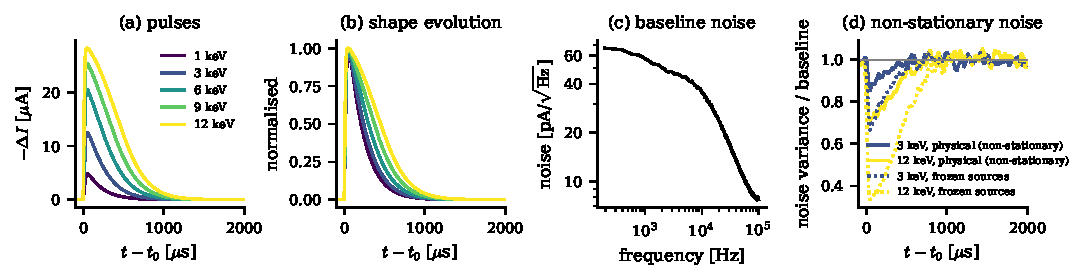
\includegraphics[width=\textwidth]{figures/pulses.pdf}
\caption{Simulated TES. (a) Mean pulses at 1--12\,keV. (b) The same, normalised,
showing saturation and the lengthening decay. (c) Baseline noise spectrum. (d) Noise
variance during the pulse relative to baseline (1500 records per curve), for the
physical model (solid) and with the noise-source amplitudes frozen at the bias point
(dotted).}
\label{fig:pulses}
\end{figure*}

\subsection{Learned subspace and manifold}
Stage A converged in \sipcaIters{} iterations (\cref{fig:manifold}). The leading
whitened basis vector is a sharpened mean pulse. The next ones encode the
lengthening decay and the changing rise, and the fourth vector holds the
high-frequency structure of the onset. Coloured back with $R_0^{1/2}$, they become
the mean pulse and its shape-variation modes in current units. The coefficients trace a smooth curve whose
transverse excursions grow with energy. The spline graph fits it with a GCV-selected
penalty, and its arc length reaches $s_{\max}=\smax$ (the SNR at about 13\,keV).

\begin{figure*}[t]
\centering
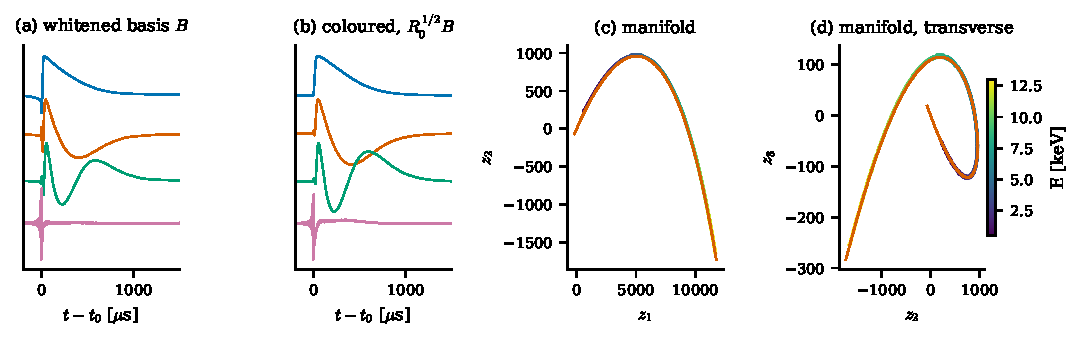
\includegraphics[width=\textwidth]{figures/manifold.pdf}
\caption{(a) Whitened shift-invariant basis ($K=4$). (b) The same vectors in the raw
domain. (c, d) Aligned coefficients of the training spectrum in the rotated frame
of the manifold, coloured by true energy, with the fitted curve.}
\label{fig:manifold}
\end{figure*}

\subsection{Structure of the pulse-correlated noise}
\Cref{fig:covariance}(a) shows the eigenvalue spectrum of the residual covariance
about the cluster means. A few eigenvalues stand far above the Marchenko--Pastur
edge~\cite{MarchenkoPastur1967} of the noise bulk, so the excess covariance is
genuinely low-rank. Correlating the mode amplitudes with the simulation truth
identifies the leading residual modes outside the signal subspace. The largest
(pooled eigenvalue $\approx$\,256) follows the sampling phase, $\sin2\pi t_0$, with
$|r|\approx0.95$. It is half of the aliasing pair of the pulse onset, which no
Fourier-shifted template can represent; its partner lies largely inside
$\operatorname{span}(B)$, where the signal-subspace part of $\Sigma$ models it. The
second ($\approx$\,76) is driven by the thermalisation parameter $\eta$
($|r|=0.96$--$0.99$), and the third mixes $\eta$ and phase. Beyond these, the
spectrum is at the Marchenko--Pastur edge. The physical non-stationary noise of
\cref{fig:pulses}(d) appears as \emph{reduced} variance, partly inside the signal
subspace. This is why the signal subspace is part of the covariance model
(\cref{sec:stageC}). Panel (c) shows its smallest eigenvalue falling below baseline
with energy.

\begin{figure*}[t]
\centering
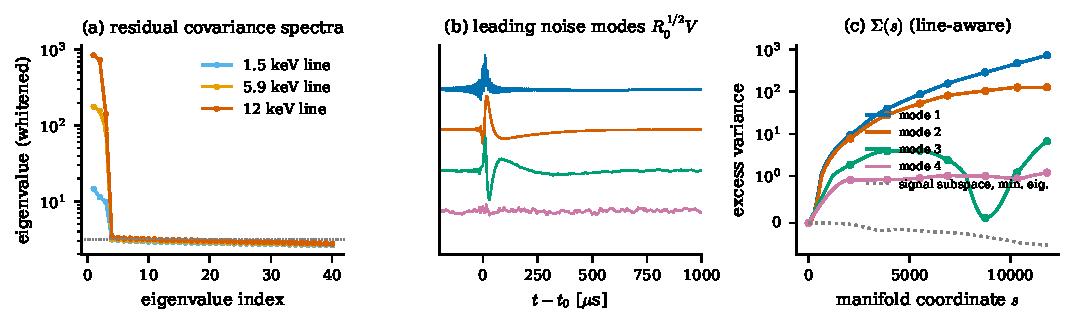
\includegraphics[width=\textwidth]{figures/covariance.pdf}
\caption{(a) Eigenvalues of the whitened residual covariance of three training lines;
dotted: Marchenko--Pastur upper edge for pure noise. (b) Leading noise modes in the
raw domain. (c) Diagonal of the interpolated excess covariance $\Sigma(s)$ (symlog
scale), with the line knots.}
\label{fig:covariance}
\end{figure*}

\subsection{Energy resolution}
\Cref{fig:resolution} and \cref{tab:fwhm} summarise the energy resolution on the
held-out test lines.

\paragraph{Against the plain optimal filter.} In scenario (a), the OF degrades from
\resOFLo{} to \resOFHi\,eV between 1 and 11\,keV, and the PCA norm behaves
similarly. The stationary manifold ML removes the template-mismatch penalty and
reaches \resStatHi\,eV at 11\,keV. Its resolution is then limited by the tangential
part of the rise-time and sampling-phase fluctuations. As
\cref{prop:identifiability} predicts, the label-free Woodbury variant leaves this
limit unchanged. The line-aware Woodbury ML removes it and reaches
\resLinesLo--\resLinesHi\,eV, a factor of \gainLo{} to \gainHi{} better than the OF.
It agrees with the oracle local Gaussian model to within \oracleGap\,eV at every
test line. That oracle uses the test line's own covariance; ours is interpolated
from training lines at other energies.

\paragraph{Against prior-art pipelines.} The comparison with a plain OF overstates
the practical gain. The practitioner's correction chain recovers most of it: OF,
phase correction, and per-line linear decorrelation against residual projectors,
interpolated in energy. That chain reaches \resPracticeHi\,eV at 11\,keV in
scenario (a). In scenario (b), phase correction alone is the best baseline
(\resPhaseHiNoMorph\,eV). Against the best of the four baselines at each line, our
estimator is level at the lowest energies and better by up to \impBestHi\% in
scenario (a) and \impBestHiNoMorph\% in scenario (b). The
advantage grows with saturation, where the shape fluctuations, the in-pulse noise
and the energy tangent interact most. The energy-dependent full-covariance filter
of Fixsen \emph{et al.} and SIRENA is the most principled baseline. It reaches only
\resCovarHi\,eV at 11\,keV in (a) and \resCovarHiNoMorph\,eV in (b), even with
Ledoit--Wolf shrinkage toward the whitened identity. About 1700 pulses per line are
too few to estimate a $1022$-dimensional covariance, whereas the $K_v\approx12$
dimensional covariance of our model is well determined. This is the practical
content of the low-rank parameterisation, beyond its speed. The stationary secant
filter, a discrete form of tangent filtering, tracks the stationary manifold ML, as
expected for two estimates of the same curve.

\paragraph{The role of the signal subspace.} A first version of our noise model used
only the $K_n$ largest residual modes. In scenario (b) it was \emph{worse} than the
phase-corrected OF at mid energies (2.14 against 2.00\,eV at 6.5\,keV), as was the
per-line oracle in the same model class. Including the signal basis $B$ in $V$
(\cref{sec:stageC}) closed the gap: 2.00\,eV at 6.5\,keV and 2.57\,eV at 11\,keV,
against 2.77\,eV before. In this simulation the in-pulse noise along the
pulse-shape directions is partly below baseline, for the electro-thermal reason of
\cref{fig:pulses}(d). A variance-ranked residual model cannot represent this, yet
it matters directly for the energy tangent. Two alternatives we tested did not
help. A multiplicative in-pulse noise gain $g(t;E)$ was worse. A full-rank shrunk
covariance was limited by sampling noise, as described above.

\paragraph{Cramér--Rao bounds.} The CRB of the learned non-stationary model predicts
the achieved widths to within about $\pm8\%$ in scenario (b) and is conservative by
up to 13\% at high energy in (a). The stationary CRB is conservative throughout,
because the in-pulse noise is partly below baseline. These are model-based
predictions, not strict bounds on the simulated process. The oracle is the practical
reference.

\begin{figure*}[t]
\centering
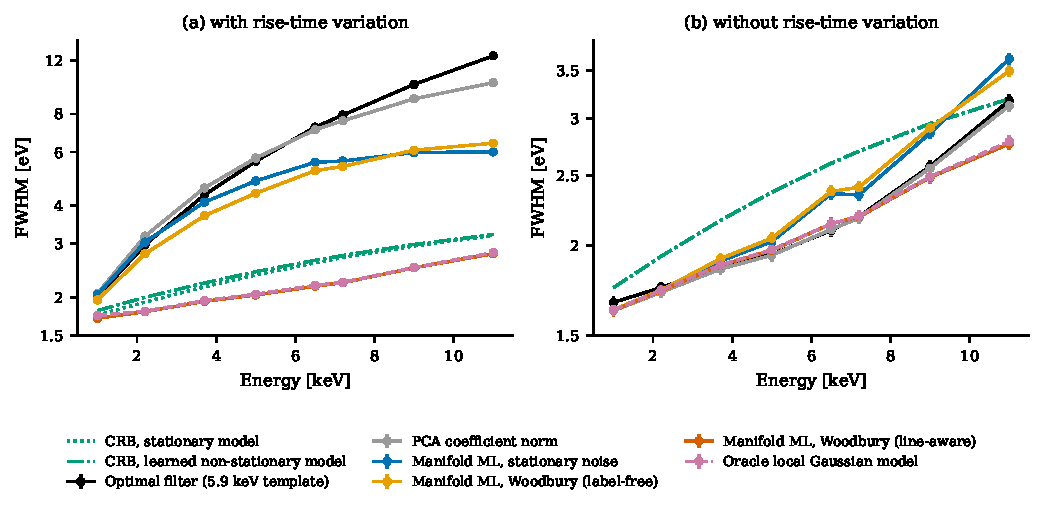
\includegraphics[width=\textwidth]{figures/resolution.pdf}
\caption{Energy resolution (FWHM) on held-out test lines that lie between the
training lines. (a) With $\pm2\%$ thermalisation-time spread; (b) without. Solid:
plain OF and the methods of this paper. Dashed: prior-art pipelines (phase-corrected
OF, OF with residual-projector decorrelation, energy-dependent full-covariance
filter) and the oracle local Gaussian model. Error bars are statistical. The plain
and phase-corrected OF coincide in (a).}
\label{fig:resolution}
\end{figure*}

\begin{table*}[t]
\centering
\caption{FWHM energy resolution [eV] on the held-out test lines.}\label{tab:fwhm}
\small
\resizebox{\textwidth}{!}{\begin{tabular}{lrrrrrrrr}
\toprule
Estimator \hfill $E$ [keV] & 1.0 & 2.2 & 3.7 & 5.0 & 6.5 & 7.2 & 9.0 & 11.0 \\
\midrule
\multicolumn{9}{l}{\emph{Scenario with rise-time variation}}\\
Optimal filter (5.9 keV template) & 2.01 & 2.98 & 4.34 & 5.60 & 7.24 & 7.93 & 9.99 & 12.40 \\
PCA coefficient norm & 2.06 & 3.18 & 4.57 & 5.73 & 7.10 & 7.59 & 8.96 & 10.13 \\
Manifold projection (Stage B) & 2.04 & 3.04 & 4.11 & 4.82 & 5.55 & 5.60 & 5.98 & 6.00 \\
Manifold ML, stationary noise & 2.04 & 3.04 & 4.11 & 4.82 & 5.55 & 5.60 & 5.98 & 6.00 \\
Manifold ML, Woodbury (label-free) & 1.96 & 2.78 & 3.71 & 4.39 & 5.21 & 5.38 & 6.08 & 6.41 \\
Manifold ML, Woodbury (line-aware) & 1.71 & 1.80 & 1.94 & 2.04 & 2.18 & 2.24 & 2.50 & 2.78 \\
Oracle local Gaussian model & 1.74 & 1.80 & 1.95 & 2.05 & 2.19 & 2.24 & 2.51 & 2.81 \\
CRB, learned model & 1.81 & 2.00 & 2.23 & 2.43 & 2.65 & 2.75 & 2.99 & 3.22 \\
\midrule
\multicolumn{9}{l}{\emph{Scenario without rise-time variation}}\\
Optimal filter (5.9 keV template) & 1.67 & 1.75 & 1.87 & 1.94 & 2.10 & 2.19 & 2.58 & 3.18 \\
PCA coefficient norm & 1.62 & 1.72 & 1.86 & 1.94 & 2.11 & 2.18 & 2.56 & 3.13 \\
Manifold projection (Stage B) & 1.63 & 1.74 & 1.90 & 2.03 & 2.36 & 2.35 & 2.86 & 3.63 \\
Manifold ML, stationary noise & 1.63 & 1.74 & 1.90 & 2.03 & 2.36 & 2.35 & 2.86 & 3.63 \\
Manifold ML, Woodbury (label-free) & 1.63 & 1.73 & 1.92 & 2.05 & 2.38 & 2.41 & 2.91 & 3.49 \\
Manifold ML, Woodbury (line-aware) & 1.63 & 1.73 & 1.88 & 1.97 & 2.14 & 2.19 & 2.49 & 2.77 \\
Oracle local Gaussian model & 1.63 & 1.73 & 1.88 & 1.97 & 2.14 & 2.20 & 2.49 & 2.79 \\
CRB, learned model & 1.75 & 1.93 & 2.17 & 2.37 & 2.60 & 2.70 & 2.95 & 3.20 \\
\bottomrule
\end{tabular}
}
\end{table*}

\subsection{Timing}
\Cref{fig:timing} compares the arrival-time jitter with the CRB. Without morphology
variation (b), the jitter equals the CRB at 1\,keV (\jitterLowE\,ns against
\crbLowE\,ns). At higher energies it levels off at \jitterNoMorphLo--\jitterNoMorphHi\,ns,
while the bound keeps falling to \crbHi\,ns. The floor is deterministic. Regressing
the timing error on three harmonics of the \emph{true} sub-sample phase removes it,
and the remaining jitter is within a factor \jitterPhaseMaxRatio{} of the CRB at
every line (\jitterPhaseHi\,ns at 11\,keV). The cause is the same residual aliasing
of the pulse onset that produces the sampling-phase noise modes: a pulse that is not
band-limited is displaced differently depending on where it falls between samples.
The low-rank covariance treats these modes as random, which is correct for the
energy estimate, but the phase-dependent displacement is a \emph{bias} in $t_0$.
Without labels, the bias is identifiable only through the
non-uniformity of the histogram of $\hat t_0\bmod1$, because true arrival phases
are uniform. A bias of amplitude $b$ makes that density non-uniform by about
$2\pi b$. Its Fourier estimate from $n$ records has standard error $\sqrt{2/n}$, so a
reliable correction needs $n\gg2/(2\pi b)^2$, about $10^5$ records for
$b\approx0.004$ samples. Equalising the phase histogram on our $\sim$1700 records per
line therefore failed: the correction added more scatter than it removed. Within
bins of a continuum it failed for a second reason, because the energy-dependent
walk smears the histogram. With enough statistics it works. On mono-energetic sets
of $10^5$ simulated records, a three-harmonic \texttt{PhaseEqualizer} learned on
\eqNmax{} records reduces the jitter at 11\,keV from \eqBefore{} to \eqAfter\,ns,
against a CRB of \eqCRB\,ns, and at 2.2\,keV from \eqBeforeLow{} to \eqAfterLow\,ns
(CRB \eqCRBLow\,ns). The residual gap to the bound at 11\,keV reflects the three-harmonic
truncation and the finite learning set. With 1000 learning records the correction
is harmful (\eqAfterSmall\,ns at 11\,keV; \cref{fig:timingeq}). Real spectra of
$10^6$ events per line make it a practical, label-free correction. At low statistics a phase-resolved manifold
$\vect c(s,\varphi)$ would be needed.

\begin{figure}[t]
\centering
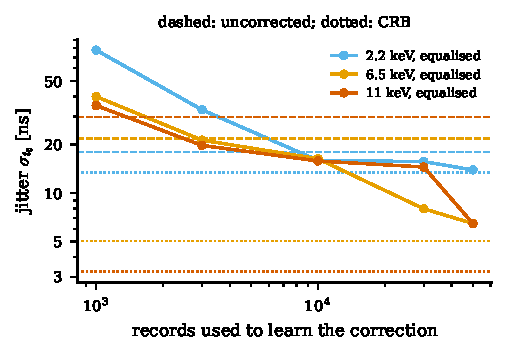
\includegraphics[width=\columnwidth]{figures/timing_equalize.pdf}
\caption{Arrival-time jitter after label-free phase-histogram equalisation, versus
the number of records used to learn it (mono-energetic simulated sets, no
morphology variation). Dashed: uncorrected. Dotted: CRB.}
\label{fig:timingeq}
\end{figure} With
morphology variation (a), all estimators sit at \jitterMorphLo--\jitterMorphHi\,ns:
a $\pm2\%$ change of the thermalisation time moves the apparent arrival time by
more than the noise does. Under shape variation the definition of $t_0$ is itself a
gauge choice (\cref{sec:discussion}).

\begin{figure*}[t]
\centering
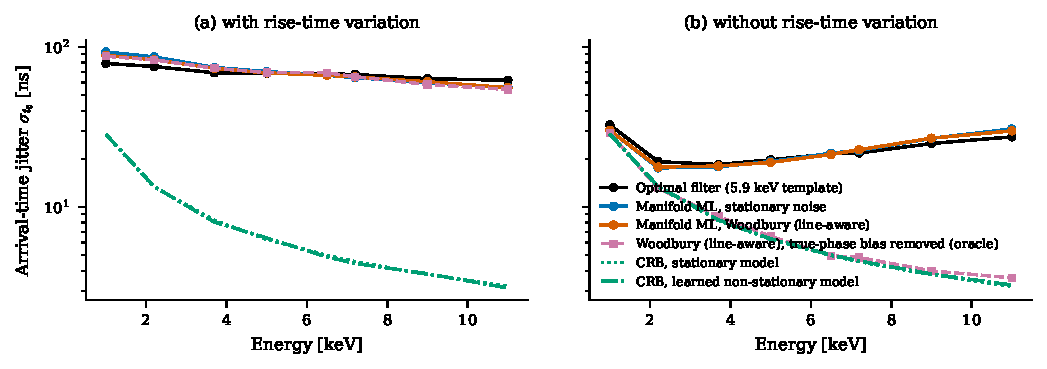
\includegraphics[width=\textwidth]{figures/timing.pdf}
\caption{Arrival-time jitter per test line (per-line time-walk offset removed;
$1\,\text{sample}=\SI{5}{\micro s}$). Dashed: line-aware ML after regressing out the
dependence on the true sub-sample phase (oracle diagnostic). Dotted and dash-dotted:
CRB of the learned stationary and non-stationary models.}
\label{fig:timing}
\end{figure*}

\subsection{Low-energy behaviour}
\Cref{fig:lowenergy} shows the response to events from 0 to 320\,eV. Each estimator
is calibrated by a quadratic through the origin fitted at 80--320\,eV, because the
detector is slightly non-linear even there. The coefficient norm is biased upward
by \normBiasZero\,eV at zero energy, and the bias decays only over the first few
tens of eV, as \cref{prop:rician} predicts. The OF with an arrival-time search is
also biased (\ofBiasZero\,eV): maximising the filter output over lags selects
positive noise excursions. The manifold ML is unbiased (\mlBiasZero\,eV), because
its search over $\tau$ is symmetric in the sign of $s$. The price is a
\mlSpreadZero{} wider, bimodal zero-energy distribution, since the free arrival
time picks the largest $|s|$ of either sign. Above a few eV all
three have the same spread.

\begin{figure*}[t]
\centering
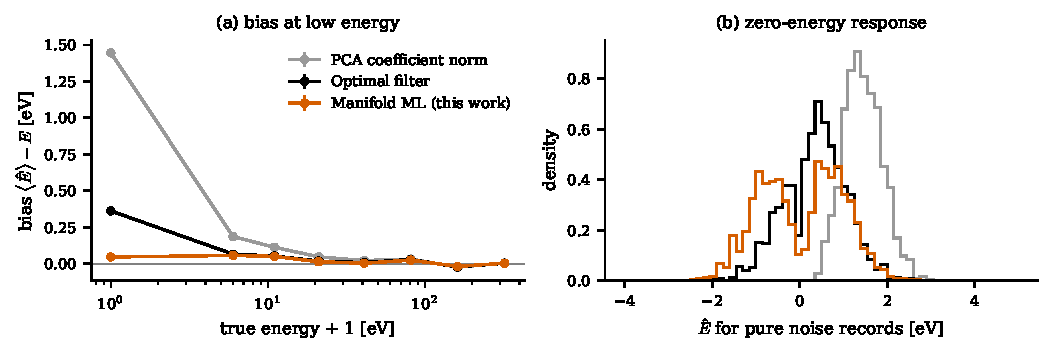
\includegraphics[width=\textwidth]{figures/lowenergy.pdf}
\caption{(a) Bias of three estimators at low energy. (b) Distribution of the
estimates for pure-noise records.}
\label{fig:lowenergy}
\end{figure*}

\subsection{Computational cost}
\Cref{fig:woodbury} compares the time per likelihood evaluation of the
$K_b$-dimensional formula~\eqref{eq:woodbury} with a dense Cholesky evaluation of
the same non-stationary model. The two agree to a relative precision of
\woodburyPrec{} for all $N$. At $N=1024$ the Woodbury evaluation is
\woodburySpeedup{} times faster per $(E,t_0)$, and the advantage grows with $N$.
The full pipeline processes \rateLines{} records/s on one CPU core for the
line-aware ML, against \rateOF{} for the OF, in our pure-NumPy implementation.

\begin{figure}[t]
\centering
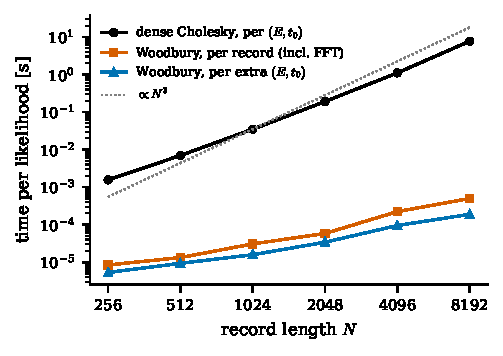
\includegraphics[width=\columnwidth]{figures/woodbury_timing.pdf}
\caption{Time per evaluation of the non-stationary log-likelihood: dense Cholesky
versus \cref{thm:woodbury} ($K_s=4$, $K_n=8$).}
\label{fig:woodbury}
\end{figure}

\subsection{Ablations}
\Cref{fig:ablation} varies $K$ and $K_n$. The resolution is insensitive to $K$
between 2 and 8: the manifold is smooth enough that two whitened components
describe it, and extra components neither help nor hurt.
With the signal subspace in the covariance, a single residual mode (the
sampling-phase mode) is not enough. From $K_n=2$, the rise-time mode is included,
the resolution reaches the oracle value, and adding more modes neither helps nor
hurts noticeably. Before the signal subspace was included, ranking residual modes by
the Gaussian likelihood gain $\lambda-1-\log\lambda$ instead of by variance helped by
1--4\% at the highest energies, because it kept some directions of reduced noise.
The signal-subspace covariance captures this physics more directly, and we keep
variance ranking for the residual modes.

\begin{figure*}[t]
\centering
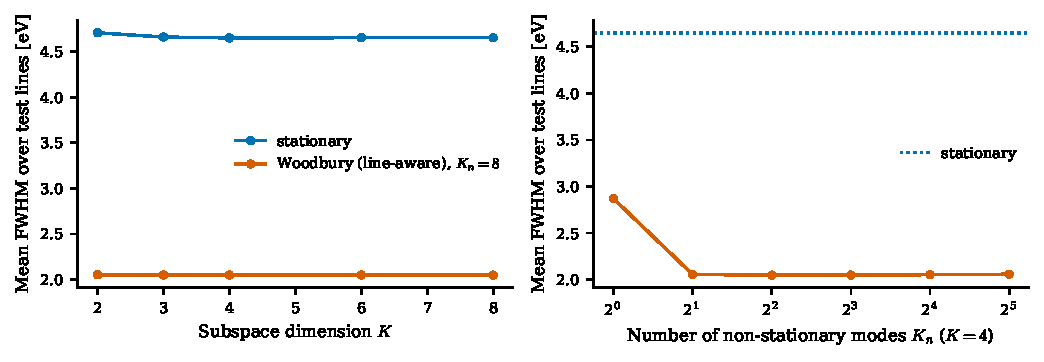
\includegraphics[width=\textwidth]{figures/ablation.pdf}
\caption{Mean FWHM over the test lines versus the subspace dimension $K$ (left) and
the number of non-stationary modes $K_n$ (right), scenario (a).}
\label{fig:ablation}
\end{figure*}

\subsection{Real TES data}
\label{sec:realdata}
We applied the same code to real data distributed with NIST's MASS
software~\cite{mass}. The pulse records come from a TES at Advanced Photon Source
beamline 29 (2015), sampled every \SI{5.12}{\micro s} with 1024 samples, and are
published there as test data for arrival-phase correction. The spectrum is
dominated by one line (the source file name suggests 600\,eV), with a sparse
low-energy tail. A separate file holds 288 pulse-free records of the same channel.
Alternate records form training and test halves, so all models are learned on
\realNtrain{} line records and evaluated on \realNtest{} others. With essentially
one line, the absolute energy scale is unknown. Each estimator's width is therefore
expressed as a fraction of the line energy, using its local gain relative to the
OF amplitude measured on the off-line tail. Corrections fitted at the line keep the
OF gain there.

With a single cluster, the manifold is the secant (\cref{sec:stageB}), and the
stationary ML coincides with the OF (\realStat\% against \realOF\% FWHM). The
phase-corrected OF reaches \realPhase\%, and adding residual-projector
decorrelation with a robust (trimmed) fit reaches \realDecor\%. The line-aware
Woodbury ML reaches \realOurs$\pm$\realOursErr\%: \realImpOF\% better than the OF
and \realImpBest\% better than the best empirical correction chain, against a
baseline-noise limit of \realLimit\% (\cref{fig:realdata}). If the line is at
600\,eV, this is \realOursEV\,eV against \realPhaseEV\,eV for the phase-corrected
OF. Two lessons came from these data. First, the curve must not be fitted to the
scatter inside a line. Before the cluster-mean rule was introduced, the spline
followed the phase-driven scatter and the manifold estimator was four times worse
than the OF. Second, projector regressions must be robust to pile-up. An ordinary
least-squares fit made that baseline worse than the plain OF. This single-line set
does not test the non-linear energy manifold itself. That requires multi-line or
continuum data.

\begin{figure}[t]
\centering
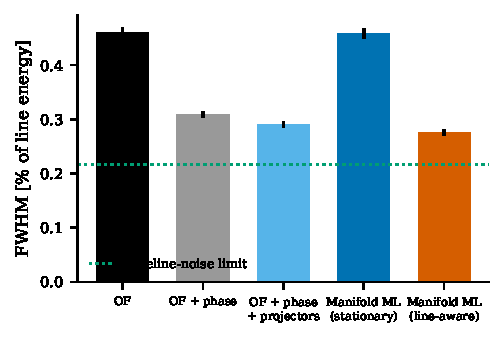
\includegraphics[width=\columnwidth]{figures/realdata.pdf}
\caption{Line width on held-out records of real NIST TES data, as a fraction of
the line energy. Dotted: baseline-noise limit of the OF.}
\label{fig:realdata}
\end{figure}

%==========================================================================
\section{Discussion}
\label{sec:discussion}

\paragraph{What the simulations support.} Against a plain fixed-template OF, the
template-free, line-aware estimator improves the FWHM by \gainLo{} to \gainHi{} on
held-out lines of a saturating TES with a $\pm2\%$ thermalisation spread. Against the
best of four prior-art pipelines it is level at low energy and up to
\impBestTopMorph\% better at the highest energies. It matches a per-line oracle
Gaussian model to within \oracleGap\,eV and needs far fewer calibration pulses than
an energy-dependent full-covariance filter. The low-energy biases of the
coefficient norm and of the OF with time search are removed. Without morphology
variation, timing reaches the CRB once a deterministic sampling-phase bias is
removed. The non-stationary likelihood costs about as much as a stationary filter
with $K_b$ templates. The method's value is therefore less a large resolution gain
over the best practice than the fact that it reaches and slightly exceeds that
practice from a single, template-free likelihood. That likelihood also yields
arrival times, Cramér--Rao predictions and a goodness of fit, without hand-built
correction stages.

\paragraph{What needs qualification.} Several statements of the original research
plan have to be weakened. First, ``calibration independence'' holds for the pulse
manifold and for the noise model, which are learned from unlabelled data. The
absolute energy scale $E(s)$ still needs reference lines, and the tangential part
of the covariance needs mono-energetic clusters (\cref{prop:identifiability}).
Second, Cholesky pre-whitening must be replaced by the symmetric spectral root for
shift invariance to be exact (\cref{lem:commute}). Third, the cost of the
non-stationary likelihood is $\mathcal O(N\log N)$ per record for the transform,
plus $\mathcal O(K_bN)$ per continuous $(E,t_0)$ evaluation (or
$\mathcal O(K_b K_n)$ once the projections are tabulated). It is not
$\mathcal O(N\log N)$ for the inverse itself, which is never formed. Fourth, the CRB of the learned low-rank model is a model-based prediction, accurate
to roughly 10\% here, not a strict bound on the physical process. Fifth, the ``$>2\times$ FWHM improvement in saturated regimes''
holds only against a plain OF and only when shape fluctuations such as position
dependence or sampling-phase effects are present. Against phase correction and
projector decorrelation, the gain is at most \impBestTopMorph\%. For a detector whose
pulses form a strict one-parameter family, a fixed template with a non-linear gain
curve loses at most \gainMaxNoMorph{} in our simulation. Sixth, sub-sample timing ``locked to the Fisher
limit'' needs a correction of the sampling-phase bias. Phase-histogram
equalisation achieves it without labels, but only with of order $10^5$ records per
energy.

\paragraph{Timing gauge.} With energy-dependent shapes, ``arrival time'' is defined
only up to an energy-dependent offset $\delta(E)$ (time walk): the reparameterisation
$\vect\mu(s)\mapsto\Sh{\delta(s)}\vect\mu(s)$, $t_0\mapsto t_0-\delta(s)$ leaves the
likelihood unchanged. Our gauge aligns the mean-pulse direction. A Fisher-orthogonal
gauge, in which $\langle\vect\mu',D\vect\mu\rangle=0$, would decorrelate energy and
time estimates. A physical onset gauge needs an external timing reference. Because
the noise-free manifold is known, conversion between gauges is a deterministic
post-processing step.

\paragraph{Limitations and outlook.} The non-linear regime is tested only in
simulation. The real-data test of \cref{sec:realdata} covers a single line and
confirms the shift-invariant learning, the line-aware covariance and its
robustness. Next, the method needs multi-line or continuum data from saturating
arrays with pile-up, gain drift and non-Gaussian tails in the shape fluctuations. Pile-up rejection can use the likelihood
value~\eqref{eq:woodbury} directly. Gain drift enters as a slow reparameterisation
of $s$ and could be tracked by line centroids. Continuous morphology parameters
could be estimated explicitly with a two-dimensional manifold
$\vect c(s,\eta)$; we did not pursue this because the tangential identifiability
problem applies there too, and the line-aware covariance already reaches the oracle.
The low-rank model would fail for noise whose non-stationarity is spread over many
modes. A diagonal-plus-low-rank model in the time domain would keep part of the
speed-up.

%==========================================================================
\section{Conclusion}
We have presented a template-free pulse processing chain for non-linear
microcalorimeters. Its three stages are shift-invariant PCA in the whitened domain,
an arc-length spline manifold, and a Woodbury-accelerated, low-rank non-stationary
maximum likelihood. Each stage optimises a stated likelihood, and each builds on an
identifiable line of prior work (\cref{sec:related}). On held-out lines of a
physically simulated, saturating TES, the chain reaches the resolution of an oracle
Gaussian model. It is level with the best empirical correction chain at low energy
and up to \impBestTopMorph\% better at high energy, at the cost of a small bank of
templates and with far fewer calibration pulses than a full-covariance filter. The
open-source implementation is intended to make these methods easy to test on real
detector data. A first test on single-line NIST TES data confirms the gain over the
best empirical correction chain. Multi-line data from saturating arrays are the
necessary next step.

\section*{Data and code availability}
All code, including the simulator and the scripts that produce every figure and
number in this paper, is available at \url{https://github.com/ytcs/empca}.

\appendix
\section{Software}
\label{app:software}
The package \texttt{empca} (import name) implements every component as a
separate, tested class: \texttt{StationaryNoise}, \texttt{ShiftInvariantPCA},
\texttt{PulseManifold}, \texttt{LowRankNoise}, \texttt{ManifoldFitter} and
\texttt{OptimalFilter}. A pipeline object chains them:
{\footnotesize
\begin{verbatim}
from empca import PulseProcessor
proc = PulseProcessor(n_components=4, n_lines=7,
                      n_noise_modes=8)
proc.fit(train_records, noise_records)
res = proc.transform(records)  # res.s, res.t0
proc.calibrate(proc.line_centers_, line_eV)
energy = proc.energy(res.s)
fwhm = proc.resolution(res.s)  # learned-model CRB
\end{verbatim}}
\texttt{PhaseEqualizer} implements the label-free sampling-phase correction of
\cref{sec:results}. The frequency-domain EM-PCA of Ref.~\cite{Yu2019} remains
available as \texttt{empca.EMPCA}.

\bibliographystyle{apsrev4-2}
\bibliography{refs}
\end{document}
